\documentclass[a4paper,11pt]{article}


%%% fontenc
%\usepackage{fontspec,xunicode,xltxtra}
%\setmainfont{Times New Roman}
%\setsansfont{Source Sans Pro}
%\setmonofont{Source Sans Pro}

%%% xeCJK
\usepackage{xeCJK}
\setCJKmainfont[BoldFont=Adobe Heiti Std]{Adobe Song Std}
\setCJKsansfont[BoldFont=Adobe Heiti Std]{Adobe Song Std}
\setCJKmonofont[BoldFont=Adobe Heiti Std]{Adobe Song Std}
\XeTeXlinebreaklocale "zh"
\XeTeXlinebreakskip=0pt plus 1pt minus 0.1pt

\usepackage{xcolor}
\usepackage{graphicx}

%%% get total page number
\usepackage{lastpage}

%%% customized definition
\makeatletter
\def\sybtitle#1{\def\@sybtitle{#1}}
\def\sybauthor#1{\def\@sybauthor{#1}}
\def\sybdate#1{\def\@sybdate{#1}}
\sybtitle{}
\sybauthor{}
\sybdate{}
\def\sybmaketitle{
  \begin{center}
  \vspace*{.8in}
  {\huge\bfseries\@sybtitle}
  \par
  \vspace{.8in}
  {\Large\@sybauthor}
  \par
  \vspace{.2in}
  \@sybdate
  \vspace{.5in}
  \end{center}
}
\makeatother
\setlength{\parindent}{0pt}
\renewcommand{\today}{\number\month 月 \number\day 日, ~\number\year 年}
\def\lt{\textless}
\def\gt{\textgreater}
\renewcommand\contentsname{\bfseries 目~~录}
\newcommand\bs{\texttt{\symbol{'134}}} % input backslash sign
%\newcommand\bs{\string\} % same as above definition
\long\def\cmd#1{\par\vspace{.5em}\hspace*{2em}#1\vspace{.5em}\par}
\def\cstr#1{\texttt{\string#1}} % e.g. \cstr{\latex}
\long\def\runcode#1{\par\bigskip#1\bigskip\par}
% 我不想看到那么多的underful hbox,尤其是minted环境加上背景色之后
\hbadness=10000
% 适当放宽overful hbox的限制,运行2pt的溢出
\hfuzz=2pt
\parskip=3\lineskip


%%% change background color & add frame for enumerate enviroment
\usepackage{mdframed}
\newmdenv[backgroundcolor=blue!10,linewidth=0pt]{coloredframe}
\newenvironment{coloredenumerate}{
  \begin{coloredframe}
  \begin{enumerate}
}{
  \end{enumerate}
  \end{coloredframe}
}

%%% geometry
\usepackage[includehead,includefoot,hmargin=21mm,vmargin=10.5mm,
            headsep=12pt,headheight=25pt]{geometry}
%\usepackage[includehead,includefoot,hmargin=1.2in,vmargin=1in]{geometry}

%%% fancyhdr
\usepackage{fancyhdr}
\makeatletter
\fancypagestyle{main} {
  \fancyhf{} % clear header & footer
  \fancyhead[L]{\bfseries\@sybtitle}
  \fancyhead[R]{\thepage/\pageref*{LastPage}}
  \renewcommand{\headrulewidth}{0.4pt} % header line
  \renewcommand{\footrulewidth}{0pt} % footer line
}
\fancypagestyle{header} {
  \fancyhf{} % clear header & footer
  \fancyfoot[C]{\roman{page}}
  \renewcommand{\headrulewidth}{0pt} % header line
  \renewcommand{\footrulewidth}{0pt} % footer line
}
\makeatother

\usepackage{titlesec}
\titleformat{\part}{\centering\Large\bfseries}{第\,\thepart\,部分}{1em}{}
\titleformat{\section}{\large\bfseries}{\thesection}{1em}{}
\titleformat{\subsection}{\normalsize\bfseries}{\thesubsection}{1em}{}
%\titlespacing*{章节命令}{左边距}{上文距}{下文距}[右边距]
\titlespacing*{\section}{0pt}{2\baselineskip}{\parsep}


\usepackage{hyperref}

%%% perfect source code display
\usepackage{minted}
%\usemintedstyle{colorful}
\definecolor{srcbg}{rgb}{0.95,0.95,0.95}
\newminted{java}{linenos,tabsize=4,bgcolor=srcbg}
\newminted{xml}{linenos,tabsize=4,bgcolor=srcbg}
\newminted{cpp}{linenos,tabsize=4,bgcolor=srcbg}
\newminted{bash}{linenos,tabsize=4,bgcolor=srcbg}
\newminted{latex}{linenos,tabsize=4,bgcolor=srcbg}
\newminted{scheme}{linenos,tabsize=4,bgcolor=srcbg}

\usepackage{amsmath}


\input{../styles/tikz_preamble}

\sybtitle{Algorithm Notes}
\sybauthor{孙延宾}
\sybdate{\today}

\begin{document}
  \tt % I love Typewriter font.
%%%%%%%% the title page and toc %%%%%%%%%%
  \pagestyle{header}
  \sybmaketitle
  \tableofcontents
  \newpage

%%%%%%% the main content %%%%%%%%%
\pagestyle{main}
\setcounter{page}{1}

\section[rsync核心算法]{rsync核心算法}
aaa


\section[伙伴算法简易实现]{伙伴算法简易实现}
\begin{center}
  % Requires \usepackage{graphicx}
  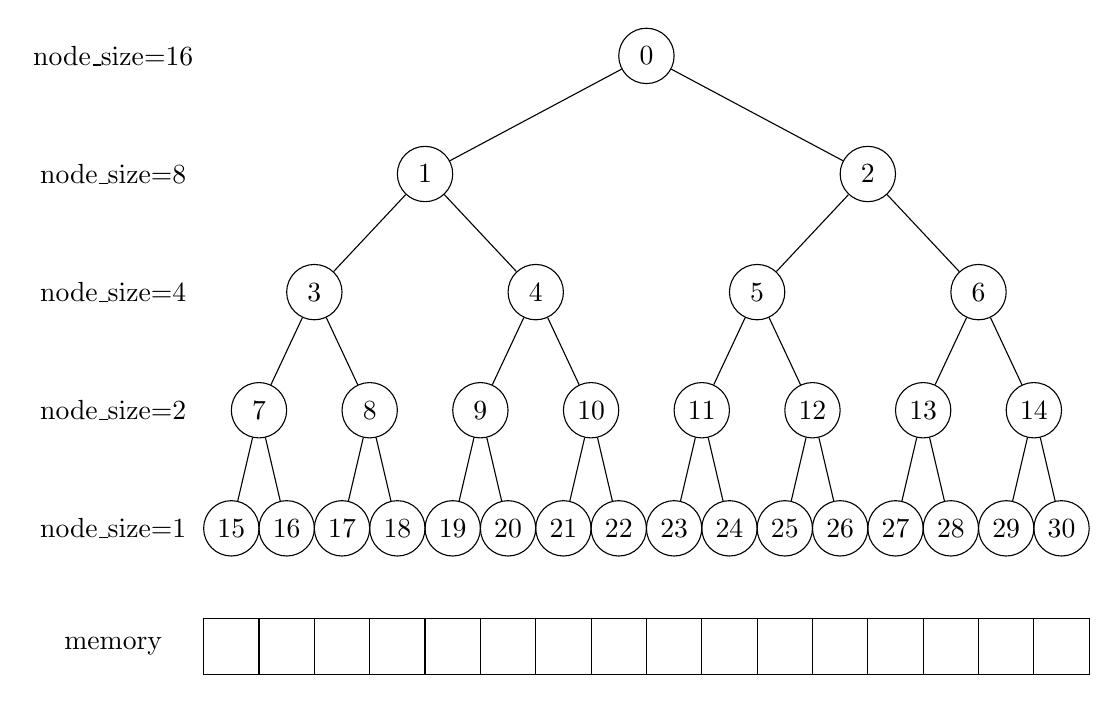
\begin{tikzpicture}
  [every node/.style={minimum size=20pt, inner sep=2pt},
   tree-node/.style={draw,circle},
   side-node/.style={},
   memo-node/.style={draw,rectangle},
   level 1/.style={sibling distance=160pt}, % 8 * 20pt
   level 2/.style={sibling distance=80pt}, % 4 * 20pt
   level 3/.style={sibling distance=40pt}, % 2 * 20pt
   level 4/.style={sibling distance=20pt}] % 1 * 20pt
  \node [tree-node] (root) {0}
    child {
      node [tree-node] {1}
        child {
          node [tree-node] {3}
            child {
              node [tree-node] {7}
                child {
                  node [tree-node] {15}
                    child [grow=down] {
                      node [memo-node] {} edge from parent[draw=none]
                        child [grow=left] {node [side-node] {memory} edge from parent[draw=none]}
                    }
                    child [grow=left] {
                      node [side-node] {node\_size=1} edge from parent[draw=none]
                        child [grow=up] {
                          node [side-node] {node\_size=2} edge from parent[draw=none]
                            child [grow=up] {
                              node [side-node] {node\_size=4} edge from parent[draw=none]
                                child [grow=up] {
                                  node [side-node] {node\_size=8} edge from parent[draw=none]
                                    child [grow=up] {
                                      node [side-node] {node\_size=16} edge from parent[draw=none]
                                    }
                                }
                            }
                        }
                    }
                }
                child {
                  node [tree-node] {16}
                    child [grow=down] {node [memo-node] {} edge from parent[draw=none]}
                }
            }
            child {
              node [tree-node] {8}
                child {
                  node [tree-node] {17}
                    child [grow=down] {node [memo-node] {} edge from parent[draw=none]}
                }
                child {
                  node [tree-node] {18}
                    child [grow=down] {node [memo-node] {} edge from parent[draw=none]}
                }
            }
        }
        child {
          node [tree-node] {4}
            child {
              node [tree-node] {9}
                child {
                  node [tree-node] {19}
                    child [grow=down] {node [memo-node] {} edge from parent[draw=none]}
                }
                child {
                  node [tree-node] {20}
                    child [grow=down] {node [memo-node] {} edge from parent[draw=none]}
                }
            }
            child {
              node [tree-node] {10}
                child {
                  node [tree-node] {21}
                    child [grow=down] {node [memo-node] {} edge from parent[draw=none]}
                }
                child {
                  node [tree-node] {22}
                    child [grow=down] {node [memo-node] {} edge from parent[draw=none]}
                }
            }
        }
    }
    child {
      node [tree-node] {2}
        child {
          node [tree-node] {5}
            child {
              node [tree-node] {11}
                child {
                  node [tree-node] {23}
                    child [grow=down] {node [memo-node] {} edge from parent[draw=none]}
                }
                child {
                  node [tree-node] {24}
                    child [grow=down] {node [memo-node] {} edge from parent[draw=none]}
                }
            }
            child {
              node [tree-node] {12}
                child {
                  node [tree-node] {25}
                    child [grow=down] {node [memo-node] {} edge from parent[draw=none]}
                }
                child {
                  node [tree-node] {26}
                    child [grow=down] {node [memo-node] {} edge from parent[draw=none]}
                }
            }
        }
        child {
          node [tree-node] {6}
            child {
              node [tree-node] {13}
                child {
                  node [tree-node] {27}
                    child [grow=down] {node [memo-node] {} edge from parent[draw=none]}
                }
                child {
                  node [tree-node] {28}
                    child [grow=down] {node [memo-node] {} edge from parent[draw=none]}
                }
            }
            child {
              node [tree-node] {14}
                child {
                  node [tree-node] {29}
                    child [grow=down] {node [memo-node] {} edge from parent[draw=none]}
                }
                child {
                  node [tree-node] {30}
                    child [grow=down] {node [memo-node] {} edge from parent[draw=none]}
                }
            }
        }
    };
\end{tikzpicture}
  %\caption{buddy system}\label{fig:buddy}
\end{center}


从伙伴算法看满二叉树的一些特性:
\begin{description}
  \item[total\_leaf\_size] 满二叉树的叶子节点总数
  \item[level] 满二叉树的层级,范围0-max\_depth
  \item[node\_size] 每个level上节点的size
  \item[index] 某个节点在满二叉树数组中的索引
  \item[offset] 某一个节点对应的内存单元映射到叶子节点数组中的下标(offset)
\end{description}
total\_leaf\_size是已知的,即buddy system管理的内存单元总数。
$$ max\_depth = \log_2total\_leaf\_size$$
每个level上第一个左子树的index为$2^{level} - 1$
\begin{align*}
  offset & = [index - (2^{level} - 1)] * node\_size \\
         & = (index + 1) * node\_size - 2^{level} * node\_size \\
         & = (index + 1) * node\_size - 2^{level} * 2^{max\_depth - level} \\
         & = (index + 1) * node\_size - 2^{max\_depth} \\
         & = (index + 1) * node\_size - total\_leaf\_size \\
\end{align*}
可见,无论哪个level,第一个左子树(最左边的节点)对应到叶子节点数组中的下标总是0.

\section[寻找小于N的所有素数]{寻找小于N的所有素数}
Sieve筛选算法用于寻找小于N的所有素数。\par
\inputminted[linenos,tabsize=4,bgcolor=srcbg]{cpp}{srcdir/Sieve.c}

筛选的方法是:\\
首先去掉2的倍数,然后去掉3的倍数,然后去掉4的倍数,然后,...,
直到去掉所有sqrt(n)的倍数,如下表:\par
\begin{tikzpicture}
\matrix [matrix of nodes]
{
  2*\textcolor{red}{2} & 3*\textcolor{red}{2} & 4*\textcolor{red}{2} & 5*\textcolor{red}{2} & $\cdots$ & $\frac{n}{2}$ \\
  2*\textcolor{red}{3} & 3*\textcolor{red}{3} & 4*\textcolor{red}{3} & 5*\textcolor{red}{3} & $\cdots$ & $\frac{n}{3}$ \\
  2*\textcolor{red}{4} & 3*\textcolor{red}{4} & 4*\textcolor{red}{4} & 5*\textcolor{red}{4} & $\cdots$ & $\frac{n}{4}$ \\
  2*\textcolor{red}{5} & 3*\textcolor{red}{5} & 4*\textcolor{red}{5} & 5*\textcolor{red}{5} & $\cdots$ & $\frac{n}{5}$ \\
};
\end{tikzpicture}

一般来说,任意一个小于sqrt(n)的数p,我们要去掉:\\
2*p, 3*p, 4*p, 5*p, $\cdots$, p*p, (p+1)*p, (p+2)*p, $\cdots$\\
观察一下可以发现,p*p以前的数字,在处理2、3、4、5、$\cdots$、(p-1)*p的倍数时
都已经去掉了,所以对于p,我们从p*p开始移除。

另外,为何只处理小于等于sqrt(n)的数字呢(上表中一直处理到n),从上面的说明可以知道,
如果$p>sqrt(n)$,$p*p>n$,无需处理,而p*p之前的数字都已经移除了,
也无需处理,所以如果$p>sqrt(n)$,则p无需处理。

该方法的缺点是占用内存太大!
\section[红黑树]{红黑树}
本节参考\href{http://zh.wikipedia.org/wiki/红黑树}{网页}。

红黑树是在二叉搜索树(Binary Search Tree, BST)的基础上增加一些性质,
从而达到自动平衡的平衡二叉搜索树(Balancing Binary Search Tree)。
它在二叉搜索树的基础上增加了如下性质,
\begin{enumerate}
  \item 节点是红色或者黑色
  \item 根节点是黑色
  \item 叶子节点是黑色(叶子节点都是NULL节点)
  \item 红色节点的两个子节点都是黑色的\\
  (即,根节点到叶子节点的路径上不能出现两个连续的红色节点)
  \item 任一节点到其每个叶子节点的简单路径包含相同数量的黑色节点
\end{enumerate}
如何理解这些性质?红黑树是为了克服BST无法自动平衡这一缺点而提出的,
所以它所增加的性质都是为了平衡性,
\begin{itemize}
  \item 前三个性质很好理解:所有节点非红即黑,上底(根节点)、下底(叶子节点)都是黑的
  \item 为了保持平衡,我们规定任一节点到每个叶子节点的简单路径有相同数量的黑色节点,
  但是这样还无法达到平衡,因为我们可以无限制的增加红色节点,所有再增加一条性质,
  \item 不能有连续存在的红色节点,这样最长路径最多是最短路径的两倍长,整棵树大致平衡。
\end{itemize}
注意:红黑树中的叶子节点指的是最末端的NULL节点。

\subsection[插入算法实现]{插入算法实现}
红黑树本质上是BST,所以插入操作首先按照BST进行插入,然后调整使之再次平衡,下面只关注如何调整。
由于任一节点到其每个叶子节点的简单路径上,黑色节点数量是相同的,所以在插入节点时
总是把新节点设置为红色,这样避免对数的结构进行调整。插入时一般分五种情况进行讨论,
\begin{enumerate}
  \item 整棵树是空的,插入的新节点作为根节点
  \item 新节点的父节点是黑色的
  \item 新节点的父节点是红色的,Uncle节点也是红色的
  \item 新节点的父节点是红色的,Uncle节点是黑色的,并且祖父节点、父节点、新节点\\
  三者是“左右”或者“右左”关系
  \item 新节点的父节点是红色的,Uncle节点是黑色的,并且祖父节点、父节点、新节点\\
  三者是“左左”或者“右右”关系
\end{enumerate}
为何会分次五种情况呢?其实这些分类是递增的,
\begin{enumerate}
  \item 新节点与其他节点没有关系(没有其他节点)
  \item 父子关系
  \item 父节点、Uncle节点、新节点之间的关系
  \item 祖父节点、父节点、新节点之间的关系(左右、右左关系)
  \item 祖父节点、父节点、新节点之间的关系(左左、右右关系)
\end{enumerate}
下面逐个情况分析对策,默认新节点颜色为红色。
\subsubsection[新节点即为根节点]{新节点即为根节点}
树是空的,所以新节点即为根节点,此时只需将新节点颜色改为黑色即可满足所有性质。

\subsubsection[父-子关系]{父-子关系}
父节点是黑色的,新节点是红色的,大家相安无事,所有性质都满足,无需任何额外操作。

\subsubsection[父-叔-子关系]{父-叔-子关系}
父节点和Uncle节点都是红色的,此时祖父节点一定是黑色的(否则之前就不是红黑树),
新节点跟父节点是连续的红色,跟性质4冲突。

我们的对策是:\\
祖父节点黑色=>红色,父节点、Uncle节点红色=>黑色,这样所有经过祖父节点的子树
仍然满足红色节点数相等(因为这些路径必定经过父节点或者Uncle节点,路径中两个节点
颜色同时翻转,黑色节点总量不变)。

但是祖父节点的父节点有可能是红色的啊,我们从祖父节点开始递归整个调整操作,
这相当于把祖父节点作为新插入的红色节点,重新进行调整。

\subsubsection[祖-父-子关系(双旋)]{祖-父-子关系(双旋)}
此时Uncle节点是黑色的,我们的调整跟他没啥关系了,我们把焦点放到祖-父-子关系上,
三者有可能是“左右”关系(即父节点是祖父节点的左子节点,新节点是父节点的右子节点)
或者“右左”关系,此时需要两次旋转来达到平衡,不过我们把一次旋转放到下一种关系中,
毕竟有些直接就是左左或者右右关系,这样就不用重复操作了。

我们的对策:\\
左右关系进行一次左旋,形成左左关系;\\
右左关系进行一次右旋,形成右右关系。

然后进入下一个情形。

\subsubsection[祖-父-子关系(单旋)]{祖-父-子关系(单旋)}
这里的情形就是“左左”或者“右右”关系,只需一次单旋,然后互换祖父节点和父节点的颜色,
所有性质再次满足。

\subsection[删除算法实现]{删除算法实现}

\subsection[时间复杂度分析]{时间复杂度分析}

\section[字符串匹配的KMP算法]{字符串匹配的KMP算法}

\section[字符串匹配的Boyer-Moore算法]{字符串匹配的Boyer-Moore算法}


\part[位操作算法实例]{位操作算法实例}

\section[Swap two numbers]{两数互换}
互换两个数的值,常规做法是使用中间变量,但是利用位操作却可以省去中间变量,
该操作与语言无关,只用到位操作“xor”,

\begin{cppcode}
// C语言版实现
int i = 42;
int j = 24;
printf("i=%d, j=%d\n", i, j);
i = i ^ j;
j = i ^ j;
i = i ^ j;
// 更加简洁的实现如下
// i ^= j = ^= i ^= j;
printf("i=%d, j=%d\n", i, j);
\end{cppcode}

原理是什么?

"xor"操作与顺序无关,即x <xor> y == y <xor> x,不过,为了便于理解,我们
称其中一个操作位为“操作因子”,

\centerline{x <xor> factor = y}

我们说:x经操作因子factor,变为y。观察factor的bit,如果是1表示“改变”,
如果是0表示“不变”,于是factor就变成了一个映射的对应关系,x、y分别是
由bit位组成的集合,并且该映射是一一对应的。

进一步,考虑到二进制的特殊性,“改变”无非就是0变1或者1变0,于是任意一个bit
经过两次“改变”就变回了自身,于是,

\centerline{(x <xor> factor) <xor> factor == x}

于是我们得出这样的结论:

\begin{cppcode}
x <xor> y = z
x <xor> z = y // x <xor> (x <xor> y) == y 经两次操作变回自身
y <xor> z = x
\end{cppcode}



\end{document}
